\section{研究工作的背景与意义}

% 3 页

互联网(Internet)是人类信息社会的标志性基础设施之一,它的出现不仅改变了人们的生活方式,也改变了人类社会的发展趋势。从一开始的电脑与电脑之间直接互相作为对等体(Peer)连接交换路由和数据,到互联网的商业化,使得能够较大范围提供互联网服务的服务器、交换机、路由器等专用设备的出现,再到近十年来云计算、物联网、大数据和分布式的人工智能系统概念兴起的背景下,互联网络的规模和复杂度日益增加。一些互联网的调研项目共同指出,广域网络(Wide Area Network)作为跨越全球各个国家和地区将若干数据中心、接入网和终端设备彼此连接的全球计算机系统,已然成为不同地域、组织和用户跨越空间限制进行信息获取和交流的主要手段\citing{douzet2020measuring} \citing{oliveira2009completeness}。它为网络带来了层次性,一定程度上简化了网络的架构,方便了网络服务商、运营商,推动了更大规模的网络发展。

广域网络本质上是一个分布式的网络系统\citing{douzet2020measuring},由不同规模的成员网络相互连接,彼此交换数据。其中,在同一行政控制下的网络路由器组成的一组网络通常拥有相同或相似的路由表、路由选择策略和网络参数,这样的一组网络在广域网际路由协议\citing{rekhter2006border}中被称为自治系统(Autonomous System,AS),是互联网中广域网的基本组成单元。这些自治系统被互联网资源管理机构赋予了唯一的自治系统号(ASN),用于在全球范围内标识和识别该自治系统。

除了最广泛被应用的互联网(同时也是目前最大的广域网络),不少社区组织和科研机构都会自发地组建不同于互联网的分布式网络,它们的管理方式和结构与互联网有着较大的差异:据现有资料显示,一些社区网络提供比互联网更加开放、灵活的连接方式\citing{tsai2022design},从而形成截然不同的拓扑结构。

网络数据的传输大多会以数据包的形式在网络上进行传输,在进入广域网的范畴后,它通常需要经过许多归属不同自治系统的路由器的中转才能抵达最终的目的地。这些路由器即是自治系统中路由功能的最小组成单元\citing{douzet2020measuring},它们在接受到数据包后,会根据内部的路由规则将其进行处理,并转发到下一个路由器\citing{aweya2001ip}。 在这个过程中,路由器之间需要通过一种或多种协议进行协作,以保证数据包能够以最快、最稳定的方式传输。

为了确定数据包传输的最佳路径,路由协议被用来进行路由选择。自治系统内的路由器通过内部路由协定(如 OSPF、IS-IS、Babel 等)共享路由信息,而不同自治系统之间的路由信息则通过边界网关协定(BGP)\citing{rekhter2006border}进行交换。 BGP 使用了许多因素来决定数据包的最佳路径,如最短自治系统路径、最低成本或是最可靠的链路等。BGP 协议的路由选择中最重要的指标是最短自治系统距离,它用于衡量从当前网络抵达目的自治系统的路线上,基于自治系统衡量的最短逻辑距离\citing{aweya2001ip}。这种路径选择方式无法达到物理距离的最优解,然而根据在实际网络传输业务的数据调研\citing{feamster2004model}中发现的结果,在政策和线路利用率约束下,逻辑上的最优方案能够有效地减少延迟和网络拥塞,从而提高网络的传输效率。

一种简化了的广域网流量路径如图 \ref{c1_wan-flow} 所示,位于自治系统 A 的终端设备发送数据包至位于自治系统 B 的终端设备,路由器 $A_i$,$B_j$ 分别为自治系统 A、B 的其中一对边界路由器。数据包在首次经过边界路由器后即进入广域网络的范畴,根据边界网关协定的路由规则被转发,直至第二次穿过边界路由器,进入自治系统 B 中,并通过内部网络抵达目标地址。

\begin{figure}[h]
    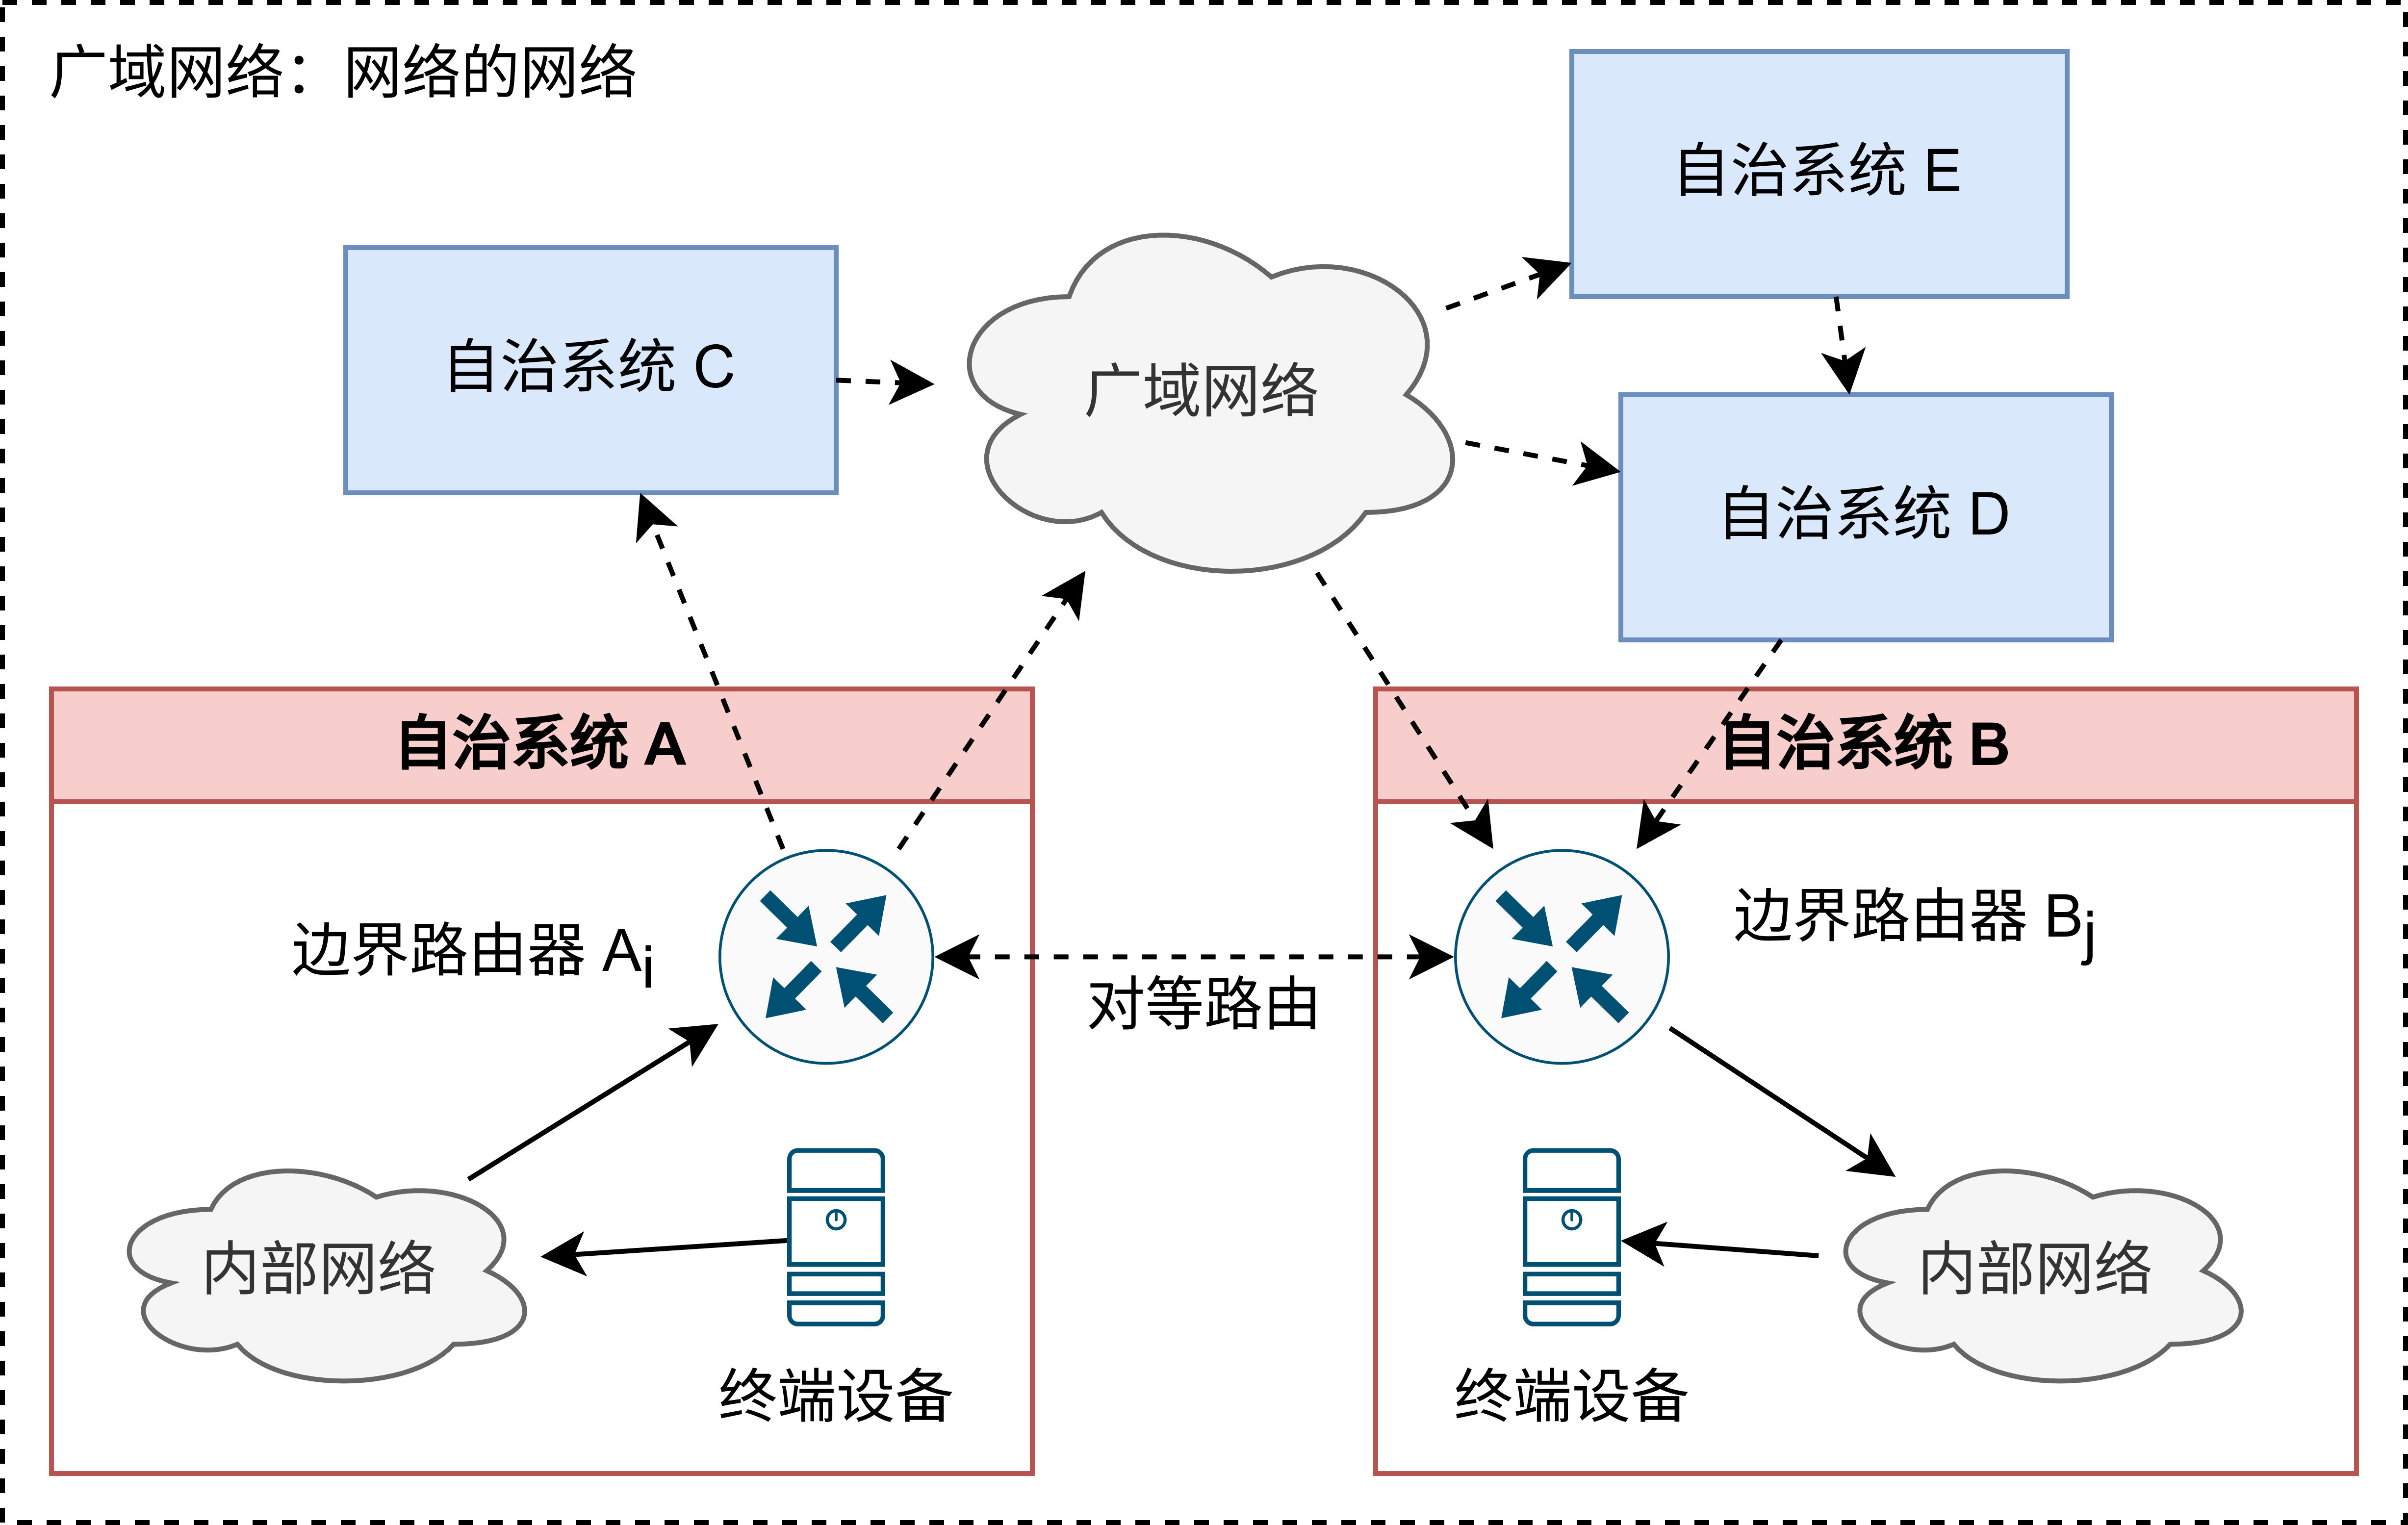
\includegraphics[width=0.7\linewidth]{chapter/c1_images/c1_wan-flow.png}
    \caption{流量途径局域与广域网络}
    \label{c1_wan-flow}
\end{figure}

在实际应用中,BGP 会通过 TCP/IP 协议相互交换并转递路由信息\citing{rekhter2006border},藉此了解其他自治系统之间的网络拓扑和路由策略,从而进行合理的路由选择。同时,由于路由表的开放性允许同一个网络被不同的运营商宣告为不同的路径,BGP 能够支持多路径路由\citing{feamster2004model},即在数据包传输过程中,可以选择多个路径进行传输,有研究指出此种路由方式提高了传输的可靠性和鲁棒性\citing{augustin2010measuring},也为提供全球性互联网服务提供了便利。 

然而,正是由于广域网结构的分布式和松散的特点,BGP 协议的核心机制中存在着一些固有的缺陷,例如在一项研究中总结的,其交换信息不受限制,而且没有强制的身份验证\citing{butler2009survey},使其在面对错误配置、异常行为或劫持攻击的情形下极为脆弱:BGP 路由信息能够在传递过程中任意修改,使得原本流向目的地的数据流量能够被不加验证地重定向到其它位置,在蓄意策划的异常情况下,能够使得攻击者不需要对目标网络系统做出任何改动即可截获和提取流量中的敏感信息。

BGP 路由异常对网络的影响也是全球性的,它可能会导致许多严重后果,如大规模的服务中断、网络可用性降低和网络失去信任等,最终影响整个广域网的连通性、稳定性和安全性,这引起了网络运营商和网络管理机构的重视,一些与网络安全相关的研究多次指出了这一点\citing{butler2009survey}。以下是几次具有代表性、影响较大的互联网路由异常的例子:

\begin{enumerate}
    \item 2008年,巴基斯坦的电信公司意外地劫持了互联网的很大一部分(包括谷歌、雅虎和其他主要网站)的流量。这是由一个配置错误的 BGP 路由器造成的,该路由器向互联网的其他部分公布了错误的路由信息\citing{ripe2008youtube}。
    \item 2010年,内容分发网络(CDN)供应商 Akamai 经历了一次BGP劫持,将本应到达其客户网络的流量被重定向到不同的地方\citing{hiran2013characterizing},导致服务中断和客户对网络失去信任。
    \item 2020年,一个BGP劫持事件影响了美国、欧洲和中东的互联网流量,将用于谷歌和亚马逊的流量重定向到不同的位置。这是由中国的一个错误配置的BGP路由器造成的\citing{graham2020cloudflare}。
    \item 2022年,一次BGP劫持被用来将加密货币交易所的流量重定向到不同的位置,使攻击者能够拦截敏感数据并窃取加密货币\citing{siddiqui2022klayswap}。此事故及其导致的严重损失引发了各界对广域网络路由安全的关注。
\end{enumerate}

在互联网的发展历程中,有很多用于缓解和避免路由异常的协议或方法被提出来,例如用于过滤无效路由的资源公钥基础设施(RPKI)标准 \citing{bush2013resource} 和用于降低路由更新频率、降低路由器负载的路由震荡抑制(Route Dampening)技术\citing{villamizar1998bgp}, 同时也有研究机构搭建公共的路由收集器\citing{orsini2016bgpstream},以此发布公开可用的数据集\citing{mao2003bgp},并提供基于不同指标的路由异常检测方案。

然而,上述方法并不能彻底解决广域网络中存在的安全性问题,也不足以应付复杂多变的网络环境。广域网络的策略、标准和局部拓扑结构在不同位置具有截然不同的特点,这是通过固定的度量标准难以实现的。近年以 FITI (国家未来互联网试验设施)\citing{谢高岗2012未来互联网体系结构研究综述}、DN42(42 号分布式网络)\citing{dn42us}为例的分布式网络实验系统的出现更是为现有模型的可迁移性提出了挑战\citing{tsai2022design}。

在广域网络路由中使用基于图的机器学习方法是具有一定依据的,路由协议本身即是一种图网络算法,一些路由指标能够很好地提供除图网络的拓扑结构以外的数据,同时,由于类似路由异常检测的带外程序无需直接与路由系统交互、不需要严格的收敛时间等响应要求,如何在路由异常检测上采用图网络模型是一种潜在的研究方向\citing{sanchez2019comparing}。

然而目前图模型在广域网的异常检测中应用并不广泛,由于广域网络的路由数据集的特征决定了它们无法直接在图网络模型中使用,一项调研指出当前的研究大多集中于中小型网络内部的局域网拓扑\citing{moustafa2019holistic}。

本研究将通过分析几类不同方向的图网络模型在不同规模的网络数据集上的检测效果,旨在探索图网络算法在路由异常检测中的应用,并据此构建出新颖高效的广域网路由异常检测模型,使其能够较好地利用网络路由中携带的拓扑信息。
